\chapter{Software Description}
Development of \SaltProc to enable use with \OpenMC constitutes a major portion
of this thesis. In this chapter, I will provide a high level overview
of my development process. The release
notes (\url{github.com/arfc/saltproc/releases}) contain more
details for those interested in specific API changes. 

\section{SaltProc development history}%
\label{sec:saltproc-history}

\SaltProc\cite{rykhlevskii_saltproc_2018} is an open source Python package that
simulates on-line reprocessing via a batch-wise approach\footnote{Material is
moved to or from the core at specific time intervals} in liquid-fueled
\Gls{msr}s. More precisely, \SaltProc manages material flows and separation
processes for nuclides in the fuel. \SaltProc relies on external codes to simulate
fuel depletion.

The first version of \SaltProc (v0.1) was a simple Python 2.7 package that used
\SerpentTWO for the fuel depletion simulations. A single Python file contained
all functions; separation processes applied to materials used an implicit 100\%
extraction efficiency at hardcoded cycle times \cite{rykhlevskii_advanced_2018}.
The structure of \SaltProc v0.1 did not lend itsef easily to development of more
sophisticated treatments of reprocessing. This led to the release of \SaltProc
v0.2, in which the entire codebase was refactored into an object oriented
context in Python 3. The addition of new functionality in the \verb.Process.
classes enabled more sophisticated treatment of online reprocessing using user
defined extraction efficiencies and removed the cycle time functionality\cite{rykhlevskii_fuel_2020}.

\SaltProc v0.3 saw the implementation of processes for gas sparging and
separation to more accurately simulate the \gls{msbr}, as well as additional
refactoring to better follow OOP concepts.

While v0.2 and v0.3 saw most of \SaltProc refactored for OOP, before I could
implement \OpenMC support, I needed to resolve the following issues:
\begin{enumerate}
    \item Relocate several functions for a more streamlined program flow
    \item Overhaul the \SaltProc input file format giving users more control over their simulations
    \item Generalize docstrings\footnote{Since \SaltProc was initially written as a script wrapped around Serpent2, many of the docstrings explicitly referenced Serpent2.}
    \item Improve function and variable names
    \item Add input file verification via JSON schema
\end{enumerate}
I implemented these changes as part of the 0.4.0 release. The changes in that
release changed the API, making 0.4.0 incompatible with previous versions of
\SaltProc. The benefit is that I was able to improve many systems for this
release, including:
\begin{itemize}
    \item An overhauled input file structure with new variable names that
    correspond to the class initialization variables.
    \item Version-controlled docpages
    \item Refactored main-program flow for clarity in code exploration
\end{itemize}

\section{SaltProc v0.5.0}
\label{sec:saltproc-detail}

\SaltProc v0.5.0, the most recent version of the software, contains a variety of
improvements and additions:
\begin{itemize}
    \item Full support for \OpenMC
    \item Revamped and revitalized webhosted docpages, including an
    \OpenMC-style user guide and theory manual, examples, and descriptions of
    the input and output 
    \item Adjusted input file structure to accommodate \OpenMC depletion 
    options and default values\footnote{See Appendix \ref{appex:input-files}
    for examples of the input files for versions v0.3.0, v0.4.0, and v0.5.0}
\end{itemize}

The majority of the work for implementing \OpenMC support focused on the
creation of a child class with methods for getting depletion results and
neutronics parameters from the \OpenMC simulation. The general program
flow is unchanged due to the class-based structure, which allows reuse of most
of the existing code for this feature. I encourage readers interested in
architectural and design details to reference Ryklhevskii's dissertation
\cite{rykhlevskii_fuel_2020} or the web-hosted \SaltProc docpages at
\url{arfc.github.io/saltproc}.


An important feature of the \OpenMC implementation is the use of control flow
to add nuclides in the depletion chain to depletable materials. As of \OpenMC
v0.13.3, in order to obtain reaction rate tallies for a nuclide, that nuclide
must be explicitly present in a material. For regular \OpenMC depletion
simulations, the program adds any nuclides in the depletion chain not present
in the material at a concentration of 1e-21 atom-\%. This is so any nuclides
that would be produced during the timestep have accurate reaction rates. If
these nuclides were not included, they would only be produced which is
non-physical behavior. Since there are additional removal processes in
\SaltProc, nuclides can be included in a material with zero percent composition,
which is effectively the same as not having the nuclide in a material at all. This
bypasses the \OpenMC machinery that detects missing nuclides, and will cause
the simulation to only caclulate production reactions for those nuclides.

To fix this, I introduced control flow in the main function\footnote{in hindsight,
the root of this issue lies in how materials are processed in \SaltProc, so any code
added to fix it should have gone in the Materialflow class. I have
added an issue to the repository to fix this PUT ISSUE LINK HERE}
to add these missing nuclides back in. While overall this shouldn't
significantly effect the neutronics of the simulation, it could influence the
compositions of individual nuclides present in small quantities in the
simulation, leading to massive errors in the nuclide compositon. I give
examples of some of these nuclides in Section \ref{sub:nuclide-compositons}

The behavior of depletion in \SerpentTWO is \ldots

I did make one significant change to \SaltProc as part of the v0.5.0 release
not directly related to \OpenMC support; I removed of PyNE as a dependency.
I did this to make \SaltProc easier to install, as installing PyNE alongside
\OpenMC is difficult to do unless the user is comfortable installing packages
from source. \OpenMC's \verb.Material. class replaces PyNE's \verb.Material.
class, and the SerpentTools package replaced the \SerpentTWO parsing
functionality of PyNE. I do not expect this change to introduce errors into
\SaltProc.

in the main execution function to add any missing nuclides

\section{Mathematical description of material reprocessing}
Rykhlevskii has discussed the design of \SaltProc's feeds and separations in
his dissertation qualitatively, however the existing \SaltProc literature is lacking a {\it mathematical} description of the reprocessing scheme\footnote{Luke Seifert's master's thesis does provide a general
mathematical description of batchwise reprocessing based on \SaltProc, and
compares it to continuous reprocessing, and I encourage readers to
cross-reference it against my own description. As of writing this, his thesis
has yet to be submitted and accepted.}, and to properly interpret the math, we
must first understand the design of the feeds and separations.

\subsection{Feeds and Separations}
\label{sub:feeds-separations}
\SaltProc models separations and feeds using three different data structures:

\paragraph{Material flows}
    A material flow represents a material with a given
    volume, density, temperature, and nuclide composition.
    It can also include information such as void fraction. \verb.Materialflow.
    objects contain the prior mentioned quantities as attributes, as well as
    methods to perform the following:
    \begin{itemize}
        \item Add two \verb.Materialflow. objects together
            \begin{itemize}
                \item The mass of the sum is $m_{1+2} = m_{1} + m_{2}$
                \item The composition of the sum is $N_{1+2} = \frac{N_{1} * m_{1} + N_{2} * m_{2}}{m_{1} + m_{2}}$
                \item The temperature and density are assumed to be equal to the
                    first \verb.Materialflow. object
            \end{itemize}
        \item Scale a \verb.Materialflow. object by a constant, specifically
            the mass and volume of the \verb.Materialflow. object.
    \end{itemize}
    \verb.Materialflow. objects are used to store information about materials
    in reprocessing as well as materials being fed into the system.

\paragraph{Processes}
    A process is an abstraction of chemical separation, extraction, or some
    other removal. Two processes commonly used in \Gls{msr}s include
    extracting metals using gas sparging and filtering. In \SaltProc,
    \verb.Process. objects contain data and functions to perform their
    associated processing task. At a minimum, a \verb.Process. object includes
    the following
    \begin{itemize}
        \item A mass flowrate, $\dot{m}$, that specifies the mass of fuel salt a process can operate on per unit time
        \item An extraction efficiency, $\epsilon$, for target element(s).
        \item A method to apply the process on a \verb.Materialflow. object. 
    \end{itemize}

\paragraph{Graphs}
    A graph is a mathematical object that connects {\it nodes}\footnote{the
    terms vertices and points are also used} with {\it edges}. More formally,
    a graph is a pair of sets, $(V, E)$, where
    \begin{itemize}
        \item $V$ is a set whose elements are called nodes
        \item $E$ is a set whose elements are pairs of elements in $V$
    \end{itemize}
    A directed graph is a graph in which the elements are ordered pairs of elements
    in $V$. This gives the edges a direction. \SaltProc uses directed graphs to
    model the order and path in which processes operate on materials.
        
Processes and feeds are defined in one JSON input file, and the graph linking
processes is defined in a DOT file. The process graph must be directed and
acyclic in order to work with \SaltProc v0.3.0 and above. At runtime,
\SaltProc reads this input file to create \verb.Process. objects for each item
in the file. Every process file must have at lest a \verb.core_outlet. and
\verb.core_inlet. Process.

\subsection{Material reprocessing}
Recall that \SaltProc uses a {\it batchwise} reprocessing scheme.

Let $\mathbf{n}(t)^{j}$ denote the nuclide mass vector for depletable material
$j$ as function of time. For each depletable material $j$, the depletion
solver numerically integrates the equation

\begin{equation}
    \frac{d\mathbf{n}^{j}(t)}{dt} = \mathbf{A}(\mathbf{n}^{j}(t), t)
\end{equation}

from time $i$ to time $i+1$ to get $\mathbf{n}^{j}(i+1)$, where $A$ is the
depletion matrix. This sequence is called a {\bf depletion step}.

Now, let the mass and volume of depletable material $j$ be
$m^{j}$ and $V^{j}$ respectively. Let the mass flowrate of process $p$ be
$\dot{m}_{p}$. At the end of each depletion step, \SaltProc constructs process
paths from the process graph defined in the DOT file, and sequentially applies
each process $p$ in each path $r$ to the relevant materials to obtain through
and waste streams for each material. \SaltProc tracks the mass and nuclide vector for both through and waste streams. For through
streams, \SaltProc also tracks the volume and mass flowrate. For every node
$p\in[0,l]$ where $0$ represents the core outlet and $l$ represents the core
inlet, in the path $r$, for the through streams we have

% still need burnup, temp, density, void frac
\begin{equation}
    \mathbf{n}^{j}_{\text{through, }p,r} = \mathbf{n}^{j}_{\text{through, }p-1,r} (1 - \pmb{\epsilon}^{j}_{p,r})
\end{equation}
\begin{equation}
    m^{j}_{\text{through, } p,r} = \alpha_{p} m^{j}_{\text{through, }p-1,r} - m^{j}_{\text{waste, }p,r}
\end{equation}
\begin{equation}
    V^{j}_{\text{through, }p,r} = \alpha_{p}V^{j}_{\text{through, }p-1,r}
\end{equation}
where 
\begin{equation}
    \alpha_{p,r} = \frac{\dot{m}_{p,r}}{\dot{m}_{\text{outlet}}}
\end{equation}
and the initial conditions are 
\begin{equation}
    \mathbf{n}^{j}_{\text{through, }0,r} = \mathbf{n}^{j}(i+1)
\end{equation}
\begin{equation}
    m^{j}_{\text{through, }0,r} = \rho^{j}(i+1)V^{j}(i+1)
\end{equation}
\begin{equation}
    V^{j}_{\text{through, }0,r} = V^{j}(i+1)
\end{equation}
Similarly, for the waste streams, we have
\begin{equation}
    \mathbf{n}^{j}_{\text{waste, }p,r} = \mathbf{n}^{j}_{\text{through, }p-1,r} \cdot \pmb{\epsilon}^{j}_{p,r}
\end{equation}
\begin{equation}
    m^{j}_{\text{waste, }p,r} = \alpha_{p,r} m^{j}_{\text{through, }p-1,r} \langle\mathbf{1},\mathbf{n}^{j}_{\text{waste, }p,r}\rangle
\end{equation}

\begin{figure}[htpb]
    \centering
    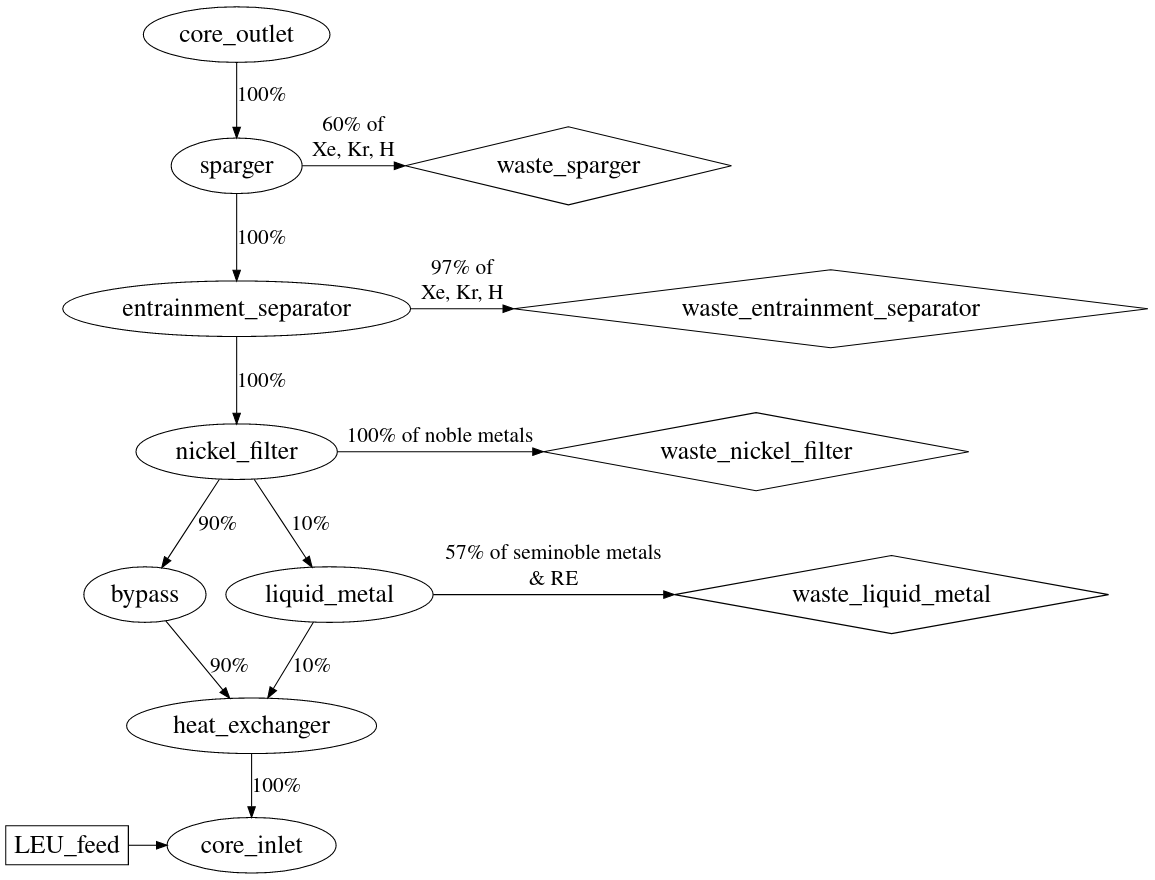
\includegraphics[width=0.8\textwidth]{figs/ch3/example_process_graph}
    \caption{Example processing system graph}
    \label{fig:example-graph}
\end{figure}

SaltProc does not currently track the volume and mass flowrate of waste streams.
In practice, since it is extremely resource intensive to separate individual
isotopes, SaltProc only allows extraction efficiencies to be defined for
elements. So for any isotope $a$ of xenon,
$\epsilon_{\ce{^{a}Xe}} = \epsilon_{\ce{^{a^{\prime}}Xe}}$  where
$a^{\prime} \in \text{isotopes of Xe}$

After the recursive computation, \SaltProc sums through and waste streams over all
paths to get the total through stream at the inlet, and the total waste stream at
the inlet which represents all material removed during reprocessing. In practice,
we are working with nuclide mass fractions, not total masses, so in the program
there is an expansion and then normalization of the vectors:
\begin{equation}
    \mathbf{n}^{j}_\text{through, inlet, net} = \frac{\sum_{r} m^{j}_{\text{through, inlet, }r} \mathbf{n}^{j}_{\text{through, inlet, }r}}{\sum_{r} m^{j}_{\text{through, inlet, }r}}
\end{equation}
\begin{equation}
    \mathbf{n}^{j}_{\text{waste, inlet, net}} = \frac{\sum_{r} m^{j}_{\text{waste, inlet, }r} \mathbf{n}^{j}_{\text{waste, inlet, }r}}{m^{j}_{\text{waste, inlet, }r}}
\end{equation}

Before running the next depletion step, for any material that has an associated
feed material defined, \SaltProc will add an amount of the feed material
equivalent to the removed mass so that the mass of fuel salt undergoing depletion
remains constant. For feed $j'$ corresponding to material $j$, we have
\begin{equation}
    \mathbf{n}^{j}_\text{filled} = \frac{m^{j}_{\text{through, }l}\mathbf{n}^{j}_\text{through, inlet, net} +  m^{j}_{\text{removed}}\mathbf{n}^{j'}}{m^{j}_{\text{through, }0}}
\end{equation}

where 
\begin{equation}
    m^{j}_\text{removed} = m^{j}_{\text{through, }0} - m^{j}_{\text{through, }l}
\end{equation}
